% Chapter X

\chapter{Assembling of a new Heat Flux Partitioning Model} % Chapter title

\label{ch:NewHFP} % For referencing the chapter elsewhere, use \autoref{ch:name} 

%----------------------------------------------------------------------------------------

\section{New model}


\section{General description of the model}
\label{sec:model}

The main goal of such a model is to provide a way to compute the wall temperature $T_{w}$ resulting from the applied wall heat flux $\phi_{w}$, or the other way around.

\npar
In order to try to be as extensive as possible regarding the different heat transfer mechanisms at stake, the wall heat flux is supposed to be split between 4 different contributions (Figure \ref{fig:HFP}) :

\begin{itemize}
\item A convective heat flux towards the liquid phase, unaffected by the presence of bubbles on the heater surface : $\phi_{c,l}$
\item A boiling heat flux, representing the energy removed from the wall to grow a bubble up to its lift-off diameter : $\phi_{b}$
\item A quenching heat flux, accounting for transient heat transfer to the liquid phase when bubbles slide or lift-off from the wall : $\phi_{q}$
\item A convective heat flux towards the vapor phase, representing the heat transfer occurring through the dry areas of the surface beneath the bubbles : $\phi_{c,v}$
\end{itemize}


\begin{figure}[h!]
\centering
\fbox{

\begin{tikzpicture}[scale=3.0]

\coordinate (O) at (0,0);
\coordinate (A1) at (1,0);
\coordinate (A2) at (2,0);
\coordinate (A3) at (3,0);
\coordinate (A) at (4,0);


%Sections and wall
\draw (O) -- (A);
\draw ($(O)-(0,0.03)$) -- ($(A)-(0,0.03)$);
\foreach \i in {0,...,19}
{
\draw (\i*0.2,0) -- (\i*0.2+0.05,-0.03);
}



%\draw[dashed, gray!70!white] (A1) --++ (0,1);
%\draw[dashed, gray!70!white] (A2) --++ (0,1);
%\draw[dashed, gray!70!white] (A3) --++ (0,1);



%Flow arrows
\foreach \i in {1,...,12} 
{
\coordinate (Oloc) at ($(O)+(-0.1,\i/13)$);
\draw[->,>=latex, gray!50!blue] (Oloc)--++({ln(1+0.05*\i)},0);
}

\draw ($(Oloc) + ({ln(1+0.05*12)},0)$) node[below right]{${\overline{U_{L}}}$};


%Liquid heat flux

\coordinate (Ophi) at (0.4,0);

\draw[->,>=latex, thick, blue!70!gray] ($(Ophi)+(0,-0.1)$)--($(Ophi)+(0,+0.1)$);
\draw ($(Ophi)+(0,-0.15)$) node{${\phi_{c,L}}$};


%Boiling heat flux
\coordinate (Ob) at (1.0,0);

\tikzmath{\alph = 40; \alphrad= \alph * pi / 180; \ray=0.15; \rayw = sin(\alphrad r) * \ray;}; %Geom values

\coordinate (Oarc) at ($(Ob)+({\ray * sin(\alphrad r)},0)$);
\shade[ball color = gray!40, opacity = 0.4] (Oarc) arc({-(pi/2-\alphrad) r}:{(pi+pi/2-\alphrad) r}:\ray);

\draw (Oarc) arc({-(pi/2-\alphrad) r}:{(pi+pi/2-\alphrad) r}:\ray);


\draw[->,>=latex, thick, brown!80!black] plot [smooth, tension=0.5] coordinates {($(Oarc)+(0,-0.1)$) ($(Oarc)+(0.05,+0.03)$) ($(Oarc)+(-0.05,+0.1)$)};

\coordinate (Oarc2) at ($(Oarc) + (-2*\rayw,0)$);
\draw[->,>=latex, thick, brown!80!black] plot [smooth, tension=0.5] coordinates {($(Oarc2)+(0,-0.1)$) ($(Oarc2)+(-0.05,+0.03)$) ($(Oarc2)+(+0.05,+0.1)$)};

\draw ($(Ob)+(0,-0.15)$) node{${\phi_{e}}$};



%Vapor convective flux
\coordinate (Ob) at (1.75,0);

\tikzmath{\alph = 40; \alphrad= \alph * pi / 180; \ray=0.2; \rw=\ray * sin(\alphrad r);};

\coordinate (Oarc) at ($(Ob)+(\rw,0)$);
\shade[ball color = gray!40, opacity = 0.4] (Oarc) arc({-(pi/2-\alphrad) r}:{(pi+pi/2-\alphrad) r}:\ray);

\draw (Oarc) arc({-(pi/2-\alphrad) r}:{(pi+pi/2-\alphrad) r}:\ray);

\draw[red, thick, densely dashed] (Oarc) --++ (-2*\rw, 0);

\draw[->,>=latex, thick, red!80!black] ($(Ob)+(0,-0.1)$)--($(Ob)+(0,+0.1)$);
\draw ($(Ob)+(0,-0.15)$) node{${\phi_{c,V}}$};



%Quenching heat flux
\coordinate (Ob2) at (2.75,0);

\tikzmath{\alph = 40; \alphrad= \alph * pi / 180;
\dalph=20; \dalphrad=\dalph*pi/180;
\alphadvrad=\alphrad - \dalphrad;
\alphrecrad=\alphrad + \dalphrad;
\ray=0.2; 
\rayadv=\ray *(1+cos(\alphrad r))/(1+ cos(\alphadvrad r);
\rayrec=\ray *(1+cos(\alphrad r))/(1+ cos(\alphrecrad r);};


\coordinate (Cb2) at ($(Ob2)+(0.03,{\ray * cos(\alphrad r)})$);
\draw[green!50!black,->, >=latex] (Cb2)--++({\ray+0.08},0); \draw ($(Cb2)+({\ray+0.08},0)$) node[above]{$\overline{U_{b}}$ }; %Bubble velocity


\coordinate (Oarc) at ($(Ob2)+({\ray * sin(\alphrad r)},0)$);

\shade[ball color = gray!40, opacity = 0.4] (Oarc) arc ({-(pi/2-(\alphadvrad)) r}:{(pi/2) r}:\rayadv) arc ({(pi/2) r}:{(pi+pi/2-(\alphrecrad)) r}:\rayrec);

\draw (Oarc) arc ({-(pi/2-(\alphadvrad)) r}:{(pi/2) r}:\rayadv) arc ({(pi/2) r}:{(pi+pi/2-(\alphrecrad)) r}:\rayrec);

\coordinate (Ob2) at (3.5,0.5);
\tikzmath{\ray=0.25;};

\shade[ball color = gray!40, opacity = 0.4] (Ob2) circle(\ray);
\draw (Ob2) circle(\ray);



\tikzmath{\rayspi=0.07;};

\draw[->,>=stealth,gray!50!blue] plot[domain=0:3.2,smooth,xshift=65,yshift=3] ({(\x *pi) r}:{\rayspi*(1-\x/6)}) ;
\draw[->,>=stealth,gray!50!blue] plot[domain=0:3.2,smooth,xshift=70,yshift=5] ({(\x *pi) r}:{\rayspi*(1-\x/6)}) ;

\coordinate (Ophisl) at ($(Oarc) - (\rayadv+\rayrec+0.05,0)$);
\draw[->,>=latex, thick, orange!90!gray] ($(Ophisl)+(0,-0.1)$)--($(Ophisl)+(0,+0.1)$);
\draw ($(Ophisl)+(0,-0.15)$) node{${\phi_{q,sl}}$};


\tikzmath{\rayspi=0.08;};

\draw[->,>=stealth,gray!50!blue] plot[domain=0:3.2,smooth,xshift=94,yshift=3] ({(\x *pi) r}:{\rayspi*(1-\x/6)}) ;
\draw[->,>=stealth,gray!50!blue] plot[domain=0:3.2,smooth,xshift=105,yshift=3] ({(\x *pi) r}:{\rayspi*(1-\x/6)}) ;


\coordinate (Ophiq) at ($(Ob2) - (0,0.5)$);
\draw[->,>=latex, thick, orange!90!gray] ($(Ophiq)+(0,-0.1)$)--($(Ophiq)+(0,+0.1)$);
\draw ($(Ophiq)+(0,-0.15)$) node{${\phi_{q,lo}}$};

\end{tikzpicture}

}
\caption{Sketch of the considered HFP}
\label{fig:HFP}
\end{figure}


The supposed mechanisms yields the total wall heat flux partioning (\ref{eq:HFP}) :

\begin{align}
\label{eq:HFP}
\phi_{w}=\phi_{c,l} + \phi_{e} + \phi_{q} + \phi_{c,v}
\end{align}


In the following subsections, we focus out analysis on each term to detail its modeling.

\npar


\subsection{Convective heat fluxes}
\label{subsec:conv_HF}

The convective heat fluxes towards the liquid phase $\phi_{c,l}$ and the vapor phase $\phi_{c,v}$ can be written using an associated heat transfer coefficient (\ref{eq:conv_HF}) :

\begin{align}
\label{eq:conv_HF}
\phi_{c,l}=\orangemath{a_{c,l}} \bluemath{h_{c,l}}\parth{\redmath{T_{w}}-\bluemath{T_{l}}} ~\text{ and }~
\phi_{c,v}=\orangemath{a_{c,v}} \bluemath{ h_{c,v}}\parth{\redmath{T_{w}}-\bluemath{T_{v}}}
\end{align}



\subsection{Boiling heat flux}

The total energy associated with the nucleation of a bubble with a volume $V_{b}$ can be expressed as $V_{b}\rho_{v}h_{lv}$. If one knows the nucleation frequency $f$ at which bubbles are generated along with the nucleation site density on the heater surface $N_{sit}$, the resulting heat flux associated with the nucleation phenomenon can thus be written as (\ref{eq:boil_HF}) :

\begin{align}
\label{eq:boil_HF}
\phi_{b}&=\bluemath{N_{sit}} \bluemath{f} \orangemath{V_{b}} \rho_{v} h_{lv}
\end{align}

\subsection{Quenching heat flux}

The quenching heat flux accounts for the transient heat transfer which occurs when cold liquid is brought close to the wall when a bubble slides or lifts-off, thus disrupting the previously established thermal boundary layer.

\textsc{Del Valle} \& \textsc{Kenning} have supposed that this kind phenomenon can be represented as a semi-infinite transient heat transfer between the liquid at $T_{l}$ and the wall at $T_{w}$. Solving the conductive heat transfer problem yields an instantaneous heat flux expressed as Eq.~\ref{eq:inst_quench_HF}.

\begin{align}
\label{eq:inst_quench_HF}
\phi_{q}\parth{t} = \frac{\lambda_{l}\parth{\redmath{T_{w}}-\bluemath{T_{l}}} }{\sqrt{\pi \eta_{l} t} }
\end{align}


Therefore, we can average this heat flux over a time $t_{w}$, during which the quenching operates, and ponderating it both by the portion of the affected heater area $a_{q}$ and the fraction of quenching time over a total bubble nucleation cycle $t_{w}f$, yielding : 

\begin{align}
\phi_{q}&=\orangemath{a_{q}} \bluemath{t_{w}} \bluemath{f} \frac{1}{\bluemath{t_{w}} } \int_{0}^{  \bluemath{t_{w}} } \frac{\lambda_{l}\parth{\redmath{T_{w}}-\bluemath{T_{l}} }}{\sqrt{\pi \eta_{l} t }} = \orangemath{a_{q}} \bluemath{t_{w}} \bluemath{f} \frac{2 \lambda_{l} \parth{\redmath{T_{w}} - \bluemath{T_{l}} } }{\sqrt{\pi \eta_{l} \bluemath{t_{w}} } }
\end{align}


\subsection{Needed closure relationships}

After expressing each heat flux components of the global partitioning, the resulting formulations yields a first list of parameters for which closure relationships (or at least precise definition) are needed. Terms previously highlighted in \textcolor{orange}{orange} will be given a specific definition, terms in \textcolor{blue}{blue} require a closure law, wall temperature is indicated in \textcolor{red}{red}.

\npar

The different terms needing further development are listed below :

\begin{itemize}
\item The fractions of the heater area ponderating convective and quenching heat transfers : $a_{c,l}$, $a_{c,v}$ and $a_{q}$(\ref{sec:geometry})
\item The convective heat transfer coefficients : $h_{c,l}$ and $h_{c,v}$ (Section \ref{sec:HTC})
\item The nucleation site density over the heater surface : $N_{sit}$ (Section : \ref{sec:NSD})
\item The nucleation frequency, which includes both the growth time $t_{g}$ (Section \ref{sec:bubble_growth}) of a bubble and the waiting time $t_{w}$ ({\color{red} Je dois encore proposer une modélisation pour $t_{w}$, à discuter}) : $f=1/\parth{t_{g}+t_{w}}$
\item The total bubble volume $V_{b}$ (\ref{subsec:geom_bub}) generated until its lift-off, thus including the modeling of the bubble lift-off diameter : $D_{lo}$ 
\item The phases temperature : $T_{l}$ (\ref{subsec:liq_temp}) and $T_{v}$ (\ref{subsec:vap_temp})
\end{itemize}


\subsection{Single Bubble Quenching Area}

\begin{align}
A_{q,1b} = &
\begin{dcases}
\pi R_{lo}^{2} & \text{if } l_{sl}\leq R_{lo}-R_{d} \\
%
\frac{1}{2}\pi R_{d}^{2} + l_{sl}\parth{R_{d}+R_{lo}} + \frac{1}{2}\pi R_{lo}^{2} & \text{if } l_{sl} \geq R_{lo}+R_{d}
%
\end{dcases}
\end{align}

Which can be re-expressed by defining ${l_{sl}}^{*}=\dfrac{l_{sl}}{R_{lo}}$ and ${A_{q,1b}}^{*}=\dfrac{A_{q,1b}}{\pi R_{lo}^{2}}$

\begin{align}
{A_{q,1b}}^{*} = &
\begin{dcases}
1 & \text{if } {l_{sl}}^{*}\leq 1- \frac{R_{d}}{R_{lo}} \\
%
\frac{1}{2}\parth{1+\parth{\frac{R_{d}}{R_{lo}}}^{2} } + \frac{{l_{sl}}^{*}}{\pi}\parth{1+\frac{R_{d}}{R_{lo}}} & \text{if } {l_{sl}}^{*} \geq 1 + \frac{R_{d}}{R_{lo}}
\end{dcases}
\end{align}
and we linearly interpolate those two expressions for the region where $1-\dfrac{R_{d}}{R_{lo}}\geq {l_{sl}}^{*} \geq 1+\dfrac{R_{d}}{R_{lo}}$.


\subsection{Bubble Growth}


The question of the bubble growth law during its lifetime including sliding is still an open question that aims to cover various types of heat transfer mechanisms:

\begin{itemize}
\item Evaporation due to superheated liquid near the bubble base ;
\item Evaporation of a liquid microlayer trapped between the base of the bubble and the wall ;
\item Condensation on top of the bubble when it reaches subcooled liquid ;
\item Convective heat transfer due to relative velocity between the bubble and the liquid.
\end{itemize}

To our knowledge, many authors that have been tackling this issue had to consider empirical or fitted parameters when trying to exhaustively account for all the above heat transfers. For instance, Zhou \cite{zhou_experimental_2020} and Yoo \cite{yoo_development_2018} have proposed growth models that consider all the previously mentioned mechanisms. However, to fully close their mathematical model, many empirical values were used such as:

\begin{itemize}
\item The ratio between the bubble projected area and the microlayer area ;
\item The fraction of bubble area facing subcooling liquid ;
\item Value of coefficients in the condensation law \cite{levenspiel_collapse_1959}.
\end{itemize}

Moreover, those models postulate the existence of a microlayer contributing to the growth while recent numerical and experimental investigations showed that the bubble may as well grow with a microlayer or in a pure contact line regime depending on the operating conditions \cite{urbano_direct_2018, bures_modelling_2021, kossolapov_experimental_2021}.

In order to assess the force modeling proposed before, we choose a simpler growth law derived from heat conduction in the superheated liquid layer \cite{plesset_growth_1954}. 

\begin{equation}
R\parth{t} = K\Ja_{w} \sqrt{\eta_{L}t}
\end{equation}
where $K$ is an adjustable constant, with a value around the unity depending on the boiling conditions, often expressed as $K=\dfrac{2b}{\sqrt{\pi}}$.  In the case of pool boiling in an uniformly superheated liquid, Plesset \& Zwick \cite{plesset_growth_1954} found $b=\sqrt{3}$, Forster \& Zuber \cite{forster_growth_1954} obtained $b=\pi / 2$ while Zuber  \cite{zuber_dynamics_1961} stated that values of $b$ should be lying between 1 and $\sqrt{3}$. More recently, Yun \etal \cite{yun_prediction_2012} used $b=1.56$. We can thus observe that $K=2$ is likely to be an upper bound value for the growth constant. This value can thus be lower in the case of subcooled flow boiling. For instance, later comparisons with experimental measurements suggest values of $K$ slightly below 1 for subcooled flow boiling (Figure \ref{fig:slide_maity}).

This type of bubble growth has been widely used, and showed good agreement with many experimental observations and is particularly valid for early growth stages or small bubbles at high pressure \cite{kossolapov_experimental_2021, plesset_growth_1954, klausner_vapor_1993}.



\subsubsection{Analytic derivation of bubble growth in a linear thermal boundary layer}

To further study the bubble growth process, we will try to derive an analytic

In this section, computations are conducted using the spherical coordinates $\left(\vect{e_{r}}, \vect{e_{\theta}}, \vect{e_{\varphi}}\right)$ with coordinates $(r, \theta, \phi)$. 

\begin{figure}[h!]
\centering
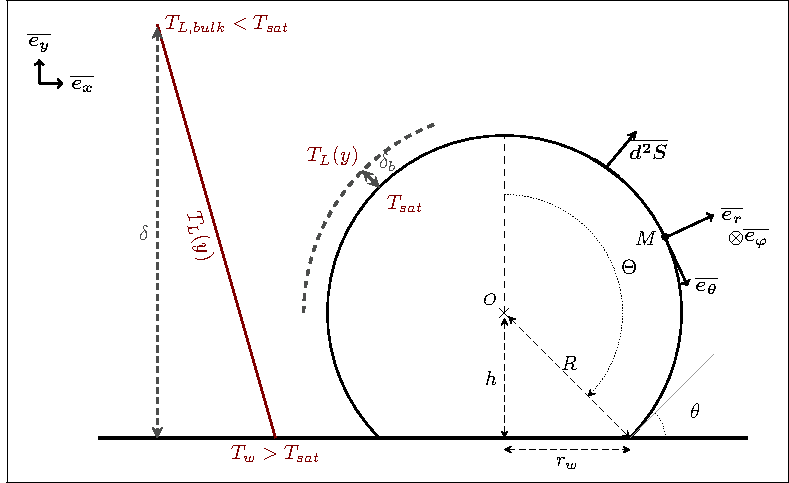
\includegraphics[width=0.7\linewidth]{img/growth/growth_analytical.pdf}
\caption{Studied geometry}
\label{fig:anal_growth}
\end{figure}

\npar
Geometrical definitions :
\begin{itemize}
\item $\Theta=\pi - \theta$ the angular portion of the truncated sphere in spherical coordinates ;
\item $r_{w}=R\sin{\theta}=-R\sin{\Theta}$ the bubble foot radius ;
\item $h=R\cos{\theta}=-R\cos{\Theta}$ the distance between the wall and the center of the bubble ($>0$ if $\theta < \pi/2$, $<0$ otherwise) ;
\item $R$ and $V=\frac{4}{3}\pi R^{3} f_{V}\left(\theta\right)$ the radius and the volume of the bubble ;
\item $\vect{d^{2}S}=R^{2}\sin{\theta}\dtheta d\varphi \vect{e_{r}}$ the surface vector in spherical coordinates ;
\item $y=R\cos{\theta}+h = R\left(\cos{\theta} - \cos{\Theta}\right)$ the distance to the wall in cartesian coordinates.
\end{itemize}


\npar
Thermal-hydraulics definitions :
\begin{itemize}
\item $\Delta T_{L} = T_{sat}-T_{\infty}$ et $\Delta T_{w}=T_{w}-T_{sat}$ the subcooling of the liquid and the wall superheat respectively ;
\item $\delta$ et $\delta_{b}$ the flow boundary layer thickness and the bubble boundary layer thickness respectively ;
\item $d^{2} Q_{b}$ the heat received by the bubble between $t$ and $t+dt$ through the surface $d^{2}S$ ;
\item $\lambda$, $\rho$, $c_{p}$, $\eta$, $h$ the thermal conductivity, density, heat capacity, thermal diffusivity and mass enthalpy respectively ($l$ standing for liquid  and $g$ for gas) ;
\item $\text{Ja}_{w}=\Delta T_{w} \rho_{L}c_{p,L}/(h_{LV}\rho_{V})$ the wall superheat (or boiling) Jakob number and $\text{Ja}_{L}=\Delta T_{L} \rho_{L}c_{p,L}/(h_{LV}\rho_{V})$ the subcooled liquid (or condensation) one.
\end{itemize}

\npar


The thermal boundary layer of the flow is assumed to follow a linear profile, giving the the expression :

\begin{align}
T_{l}\left(y\right)=T_{w}+\frac{T_{\infty}-T_{w}}{\delta} y
\end{align}


If we consider that the bubble stays at a temperature close to $T_{sat}$, the radial component of the temperature gradient at the bubble's interface yields :

\begin{align}
\grad{T} \cdot \vect{er} = \dpartial{T}{r}\left(R, \theta, \phi\right)\approx\frac{T_{\l}(y)-T_{sat}}{\delta_{b}}
\end{align}

\npar



Applying Fourier's law to the liquid close to the bubble : $\vect{j_{Q}}=-\lambda_{l} \grad{T}$, then the bubble receives between $t$ and $t+dt$ through $d^{2}S$ :

\begin{align}
d^{2}Q_{b}&=\vect{j_{Q}} \cdot \left(-\vect{d^{2}S}\right)\\
&=\lambda_{l} \dpartial{T}{r}\left(R,\theta, \varphi\right) R^{2}\sin{\theta} d\theta d\varphi\\
&\approx\lambda_{l} \frac{T_{l}\left(y\right)-T_{sat}}{\delta_{b}}R^{2}\sin{\theta}d\theta d\varphi\\
&=\lambda_{l} \frac{1}{\delta_{b}}\left[T_{w}+\frac{T_{\infty}-T_{w}}{\delta}y - T_{sat}\right]R^{2}\sin{\theta}d\theta d\varphi\\
&=\frac{\lambda_{l}}{\delta_{b}}\left[\Delta T_{w}-\frac{\Delta T_{w} + \Delta T_{l}}{\delta}R\left[\cos{\theta} - \cos{\Theta}\right]\right]R^{2}\sin{\theta}d\theta d\varphi\\
&=\frac{\lambda_{l}}{\delta_{b}}\left[\Delta T_{w}R^{2}\sin{\theta}-\frac{\Delta T_{w}+\Delta T_{l}}{\delta}R^{3}\left[\cos{\theta}-\cos{\Theta}\right]\sin{\theta}\right] d\theta d\varphi
\end{align}

\npar
The total heat flux received by the bubble can then be derived, supposing that $\delta_{b}$ is constant all around the bubble between $t$ and $t+dt$ :

\begin{align}
Q_{b}&=\int_{\varphi=0}^{\varphi=2\pi} \int_{\theta=0}^{\Theta}{d^{2}Q_{b}}\\
&= \frac{2\pi \lambda_{l}}{\delta_{b}}\left[\int_{0}^{\Theta} \Delta T_{w} R^{2} \sin{\theta}d\theta + \int_{0}^{\Theta} \frac{\Delta T_{w} + \Delta T_{l}}{\delta} R^{3} \cos{\Theta}\sin{\theta}d\theta - \int_{0}^{\Theta} \frac{\Delta T_{w} + \Delta T_{l}}{\delta} R^{3} \cos{\theta}\sin{\theta}d\theta\right]\\
&=\frac{2\pi \lambda_{l}}{\delta_{b}} \left[\Delta T_{w} R^{2} \left(1-\cos{\Theta}\right) + \frac{\Delta T_{w} + \Delta T_{l}}{\delta}R^{3}\left[\cos{\Theta}\left(1-\cos{\Theta}\right)- \frac{1}{4}\left(1 - \cos{2\Theta}\right)\right]\right]\\
&=\frac{2\pi \lambda_{l} R^{2}}{\delta_{b}}\left[\frac{-R}{2\delta}\left(\Delta T_{w} + \Delta T_{l}\right)\left(1 + 2\cos{\alpha} + \cossq{\alpha}\right) + \Delta T_{w} \left(1 + \cos{\alpha } \right) \right]\\
&=\frac{2\pi \lambda_{l} R^{2}}{\delta_{b}}\left(1+\cos{\alpha}\right)\left[\Delta T_{w} - \frac{R}{2\delta}\left(\Delta T_{w} + \Delta T_{l}\right) \left(1 + \cos {\alpha} \right )\right]
\end{align}


\npar
Between $t$ and $t+dt$, the bubble receives a $Q_{b}dt$ energy amount through thermal diffusion. Assuming this energy solely contributes to evaporation of the surrounding liquid, the resulting mass of generated vapor is :

\begin{align}
&dm_{g} = \rho_{g} dV = \frac{Q_{b}dt}{h_{lg}}\\
\text{then } &\frac{dV}{dt}=\frac{Q_{b}}{\rho_{g}h_{lg}}
\end{align}

Since $V=\frac{4}{3}\pi R^{3} f_{V}\left(\alpha\right)$, we can write : 

\begin{align}
\frac{dV}{dt}=\frac{4}{3}\pi f_{V}\left(\alpha\right) 3R^{2}\frac{dR}{dt}
\end{align}

Then :

\begin{align}
\frac{dR}{dt}&=\frac{1}{4\pi R^{2}f_{V}\left(\alpha\right)} \frac{1}{\rho_{g} h_{lg}} \frac{2 \pi \lambda_{l} R^{2}}{\delta_{b}}\left(1+\cos{\alpha}\right)\left[\Delta T_{w} - \frac{R}{2\delta}\left(\Delta T_{w} + \Delta T_{l}\right) \left(1 + \cos{\alpha} \right )\right]\\
&= \frac{1}{2f_{V}\left(\alpha\right)}\frac{\Delta T_{w}}{h_{lg}\rho_{g}}\frac{\lambda_{l}}{\delta_{b}}\left(1+\cos{\alpha}\right)\left[1 - \frac{R}{2\delta}\left(1 + \frac{\Delta T_{l}}{\Delta T_{w}}\right) \left(1 + \cos {\alpha} \right )\right]\\
&=\frac{\text{Ja}_{w} \eta_{l}}{2 \delta_{b} f_{V}\left(\alpha\right)}\left(1+\cos{\alpha}\right)\left[1 - \frac{R}{2\delta}\left(1 + \frac{\text{Ja}_{l}}{\text{Ja}_{w}}\right) \left(1 + \cos{\alpha} \right )\right]
\end{align}

If we define :

\begin{align}
a = \frac{\text{Ja}_{w}\eta_{l}}{4 \delta_{b} \delta f_{V} \left(\alpha\right)} \left(1 + \frac{\text{Ja}_{l}}{\text{Ja}_{w}}\right) \left(1 + \cos{\alpha}\right)^{2} \text{ et } b = \frac{\text{Ja}_{w}\eta_{l}}{2 \delta_{b} f_{V}\left(\alpha\right)}\left(1 + \cos{\alpha}\right)
\end{align}

Finally : 

\begin{align}
\frac{dR}{dt} + aR = b
\end{align}


\npar

Solutions of this differential equation depend on the hypothesis over $\delta$ and $\delta_{b}$. In a first approach, we will consider that $\delta$ does not vary during the whole bubble growth. This thickness could be expressed using boundary layer thickness correlations for example (laminar or turbulent depending on the Reynolds number). 

\npar

On the other hand, we will consider 3 different choices to model $\delta_{b}$ :


\npar
\subsubsection{Case 1 : $\delta_{b}$ is constant}


This is a \textbf{strong assumption} since it means that $\delta_{b}$ does not depend on the temperature and the flow shear rate facing the bubble. In this case, $a$ and be are constant, giving : 


\begin{align}
\frac{dR}{dt} + aR = b
\end{align}


With the initial condition $R(t=0)=0$ the solution of this differential equation is : 

\begin{align}
R\left(t\right)=\frac{b}{a}\left(1 - e^{-at}\right) \text{ where } \frac{b}{a} = \frac{2\delta}{\left(1 + \frac{\text{Ja}_{l}}{\text{Ja}_{w}}\right)\left(1 + \cos{\alpha} \right )}=R_{\infty} \text{ is the final bubble equilibrium radius.}
\end{align}


\subsubsection{Case 2 : $\delta_{b}=\sqrt{\eta_{l}t}$}
\npar

This expression derives from the growth of a boundary layer through pure diffusion, as studied by \textsc{Legendre} \etal

Such a boundary layer thickness is also used when one writes the quenching heat flux (see Section \ref{sec:model} and \textsc{Del Valle \& Kenning} work).

In this case, this means that the boundary layer around the bubble interface grows through diffusion only.

\npar

Thus, it yields :

\begin{align}
\frac{dR}{dt}\parth{t}+a\parth{t}R\parth{t}=b\parth{t}
\end{align}

\begin{align}
\label{eq:coeff_expgrowth}
a(t)=\frac{\Ja_{w}\sqrt{\eta_{l}}}{4\delta f_{V}\parth{\alpha}\sqrt{t}}\parth{1+\frac{\Ja_{l}}{\Ja_{w}}}\parth{1+\cos{\alpha}}^{2}=K_{a}t^{-1/2} \text{ and } b(t)=\frac{\Ja_{w}\sqrt{\eta_{l}}}{2f_{V}\parth{\alpha}\sqrt{t}}\parth{1+\cos{\alpha}}=K_ {b}t^{-1/2}
\end{align}

With the initial condition $R\parth{t=0}=0$, the solution is given by : 

\begin{align}
R\parth{t}=R_{\infty}\parth{1-e^{-2K_{a}\sqrt{t}}} \text{ avec } R_{\infty}=\frac{K_{b}}{K_{a}}
\end{align}

\npar
\subsubsection{Case 3 : $\delta_{b}=CR$}
\npar

In this last case, the bubble boundary layer is assumed to by proportional to the bubble radius $R$, through a constant coefficient $C$. This yields :


\begin{align}
a(t)=\frac{\Ja_{w}\eta_{l}}{4\delta f_{V}\parth{\alpha}CR\parth{t}}\parth{1+\frac{\Ja_{l}}{\Ja_{w}}}\parth{1+\cos{\alpha}}^{2}=K'_{a}\frac{1}{R\parth{t}} \text{ et } b(t)=\frac{\Ja_{w}\eta_{l}}{2f_{V}\parth{\alpha}CR\parth{t}}\parth{1+\cos{\alpha}}=K'_ {b}\frac{1}{R\parth{t}}
\end{align}

Giving :

\begin{align}
&\frac{dR}{dt}\parth{t} + K'_{a} = K'_{b}\frac{1}{R\parth{t}}
\end{align}

Which the solution with the initial condition $R\parth{t=0}=0$ is :

\begin{align}
R\parth{t}=R_{\infty}\parth{ \text{W}\parth{-e^{-t{K'_{a}}^{2}/K'_{b}-1} } +1}
\end{align}

With $\text{W}$ being the \textsc{Lambert} function defined as the reciprocal function of $w \rightarrow we^{w}$ on $\mathbb{C}$.


\subsection{Comparison with experimental data and DNS}

To assess the three models presented above, we compared the time-dependent radius profile given by an experiment conducted by \textsc{Maity} as shown in Figure \ref{fig:growth_comp_Maity}.


\begin{figure}[h!]
\centering
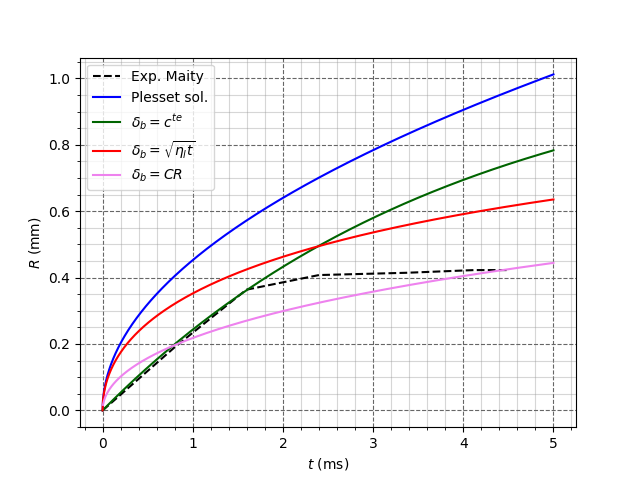
\includegraphics[width=0.7\linewidth]{img/growth/growth_maity.png}
\caption{Comparison with single bubble growth measurement from \textsc{Maity} : Boiling water at $\Delta T_{sub}=0.2\degree$C, $\Delta T_{w}=5.9\degree$C, $U_{liq}=0.23\text{~m/s}$ and $P=1\text{~bar}$. Green : $\delta_{b}=10^{-5}~$m - Red : $\delta_{b}=\sqrt{\eta_{l}t}$ - Pink : $\delta_{b}=0.1\times R\parth{t}$ - Blue : \textsc{Plesset} solution $R\parth{t}=B\sqrt{t}$ with $B=\Ja_{w}\sqrt{12\eta_{l}/\pi}$. The liquid boundary layer size has been fixed to $\delta \approx 1~$mm according to the experimental measurements.}
\label{fig:growth_comp_Maity}
\end{figure}

As we can see, the \textsc{Plesset} solution overestimates both the growth and the size of the bubble as it could have been expected since this solutions is found for a uniformly superheated liquid. Concerning the three different approaches  previously developed :

\begin{itemize}
\item The constant $\delta_{b}$ hypothesis seems to better fit the first stage of bubble growth (with an optimal choice of $\delta_{b}$ value). However, the imposed growth regime seems to large when we compare to the moderate growth of the measured bubble. Moreover, this model yields a linear start of bubble growth, while it has been thoroughly validated that under a large range of thermal-hydraulics conditions, bubble growth begins with a $\sqrt{t}$ profile.
\item The contrary is observed for the $\delta_{b}=CR$ model, with a growth being globaly too slow.
\item Choosing $\delta_{b}=\sqrt{\eta_{l}t}$ seems to better reproduce the growth regime. Even though the bubble radius is slightly overestimated, the shape of the time-dependent profile looks similar to the experimental measurement, especially since the growth is progressively damped.
\end{itemize}


To further assess the modeling, we compare the derived profiles with DNS data from \textsc{Urbano} \etal\cite{Urbano2018} on Figure \ref{fig:growth_vs_DNS}.


\begin{figure}[h!]
\centering
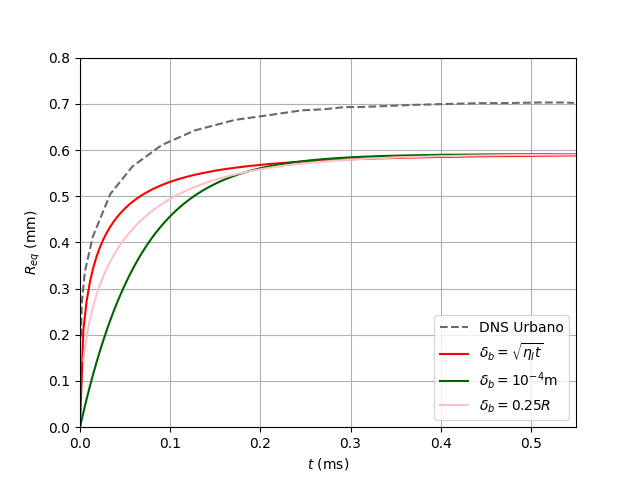
\includegraphics[width=0.7\linewidth]{img/growth/modvsDNS.png}
\caption{Comparison with zero-gravity DNS data from \textsc{Urbano} \etal : Water at $P=1.01\text{~bar}$, $\Delta T_{sub}=10\degree$C, $\Delta T_{w}=2\degree$C, $U_{liq}=0\text{~m/s}$ and $\alpha=50\degree$.}
\label{fig:growth_vs_DNS}
\end{figure}


\npar
First, it is important to note that the expression of the equilibrium radius $R_{\infty}$ matches the analytical derivation of \textsc{Urbano} \etal. Figure \ref{fig:growth_vs_DNS} shows a difference betwee, the computed equilibrium radius and the DNS equilibrium radius. This discrepancy may rely on the fact that Urbano \etal considered solid wall heat diffusion while our model considers a constant wall temperatue.

However, comparing the shapes of the predicted growth, we can see that the $\delta_{b}=\sqrt{\eta_{l}t}$ hypothesis seems to give a growth regime in accordance with the DNS results. The other hypotheses do not greatly differ, but they result from an arbitrary choice for $\delta_{b}$ or $C$. Thus, it seems appropriate to consider that the $\delta_{b}=\sqrt{\eta_{l}t}$ hypothesis is reasonable to model the evolution of the boundary layer thickness at the liquid-vapor interface.

\npar


Finally, we present on Figure \ref{fig:growth_DNS_regime} the comparison between the $\delta_{b}=\sqrt{\eta_{l}t}$ model and 3 DNS profiles for a same Jakob number ratio, but at different subcoolings and superheats. 


\begin{figure}[h!]
\begin{multicols}{2}
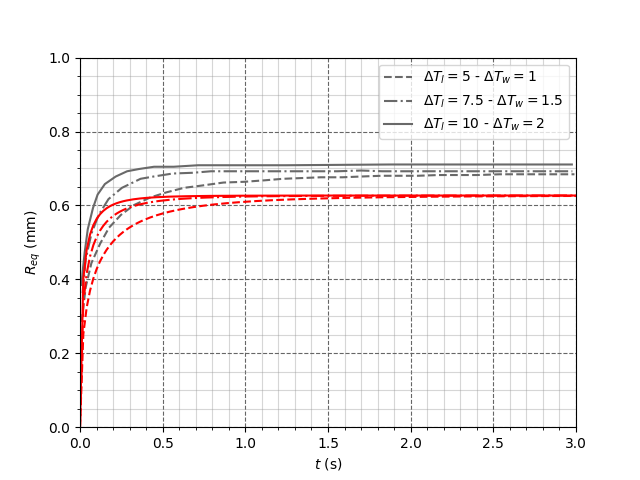
\includegraphics[width=1.0\linewidth]{img/tg/comp_Urbano.png}

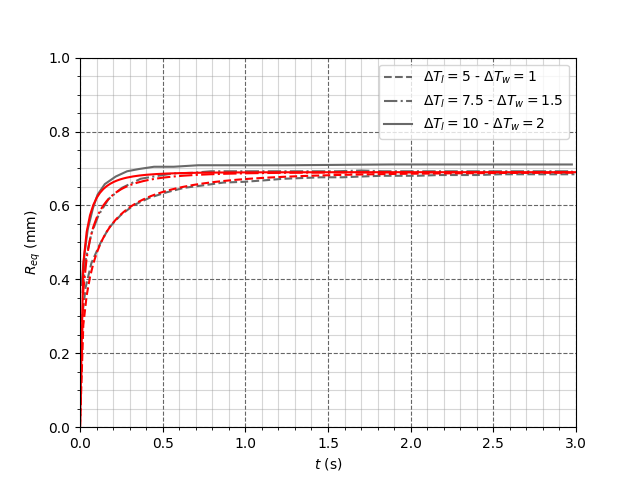
\includegraphics[width=1.0\linewidth]{img/tg/comp_Urbano_fixed_Req.png}
\end{multicols}
\caption{Comparison of the model (red) with results from Urbano \etal (gray) at 3 different pairs of $\parth{\Delta T_{l}, \Delta T_{w}}$ - Left : $R_{\infty}$ from the model - Right : $R_{\infty}$ imposed equal to the DNS}
\label{fig:growth_DNS_regime}
\end{figure}


The difference between the 3 growth regime predicted by the model is really close to the difference captured by the DNS. A discrepancy over the final equilibrium radius is still observed, but imposing the final radius from the DNS in the model yields strongly matching profiles between both approaches. 

It thus seems appropriate to consider the $\delta_{b}=\sqrt{\eta_{l}t}$ profile to represent the boundary layer thickness around the bubble.

\npar


In this case, the average radius of the bubble over a growth time $t_{g}$ (as needed in Subsection \ref{subsec:vap_area}) is :


\begin{align}
\overline{R\parth{t}}&=\frac{1}{t_{g}}\int_{0}^{t_{g}}R\parth{t} \text{d}t = \frac{R_{\infty}}{t_{g}}\crocht{ \frac{e^{-2K_{a}\sqrt{t}} \parth{2K_{a}\sqrt{t}+1}  }{2K_{a}^{2}}+ t}_{0}^{t_{g}}\\
&=\frac{R_{\infty}}{2K_{a}^{2}t_{g}}\parth{ e^{-2K_{a}\sqrt{t_{g}}}\parth{2K_{a}\sqrt{t_{g}}+1} + 2K_{a}^{2}t_{g} -1  }
\end{align}

Moreover, if we consider a lift-off radius $R_{d}$, we can express the associated growth time $t_{g}$ :

\begin{align}
t_{g}=\crocht{ \frac{1}{K_{a}}\ln{\frac{1}{\sqrt{1-\frac{R_{d}}{R_{\infty}} } } } }^{2} = \crocht{\frac{1}{K_{a}}\ln { \sqrt{1-\frac{R_{d}}{R_{\infty}} } }   }^{2}
\label{eq:growth_time}
\end{align}

This expression could then be used as a closure relationship for $t_{g}$ in the HFP model, meaning that this growth time will depend on the departure diameter closure for $R_{d}$.


\subsection{Estimation of the thermal boundary layer thickness $\delta$}

In order to fully close the modeling of the bubble growth, we have to compute the thermal boundary layer thickness $\delta$.

To do so, we test a first approach based on the hydrodynamic boundary layer profile. In the turbulent layer, the non-dimensional liquids velocity $u_{l}^{+}$ is :

\begin{align}
u_{l}^{+}=\frac{1}{\kappa} \ln{y^{+}} +B,\ \text{with}\ \kappa=0.41\ \text{and}\ B=5.25
\end{align}

Since $u_{l}^{+}\parth{y^{+}}=u_{l}\parth{y}/u_{\tau}$ and $y^{+}=yu_{\tau}/\nu_{l}$, we can compute the height of the hydrodynamic boundary layer $\delta_{h}$ where $u_{l}\parth{\delta_{h}}=0.99u_{l,bulk}$ as :

\begin{align}
\delta_{h}=e^{\kappa \parth{0.99u_{l,bulk}\sqrt{\rho_{l}/\tau_{w}}-B}}\times \nu_{l}\sqrt{\frac{\rho_{l}}{\tau_{w}}}
\end{align}

where $\tau_{w}$ is computed using the Mac Adams correlation (Eq. \ref{eq:MacAdams}).

\npar

Finally, to get an approximation of the thermal boundary layer thickness, we consider a simple first approach as :

\begin{align}
\delta=\frac{1}{\Pr_{l}}\delta_{h}
\end{align}

Since the Prandtl number is the ratio of momentum diffusivity to thermal diffusivity, its inverse shall approximately scale the ratio between the thermal boundary layer and hydrodynamic boundary layer thickness. 

\npar

\subsection{Estimation of $t{g}$ against experimental data}

In order to assess the proposed approach to compute $t_{g}$, we compare the yielded results with data taken from Unal of maximum bubble growth. 

\npar

Only 6 measurements of maximum growth time are available ({\color{red} Je vais en ajouter d'autres par la suite}) but they are associated with the bubble lift-off diameter. Since those measurements were conducted with boiling water on stainless steel, we set the contact angle at $\alpha=80\degree$.

\npar

We also compare the predictions with the model proposed by Kommajosyula :

\begin{align}
t_{g}&=\parth{ \frac{D_{d}}{4K}}^{2}\\
K&=\frac{\sqrt{\eta_{l}} \Ja_{w}}{0.804\sqrt{\Pr_{l}}}+\chi 1.95\Ja_{w} \eta_{l},\ \text{with}\ \chi=A-B\zeta
\end{align}
where $\zeta=\Ja_{l}/\Ja_{w}$ and both $A=1.55$ and $B=0.05$ have been fitted over the data of Klausner by Mazzocco \etal.

\npar

The results are displayed on Figure \ref{fig:comp_modelKomm}.

\begin{figure}[h!]
\centering
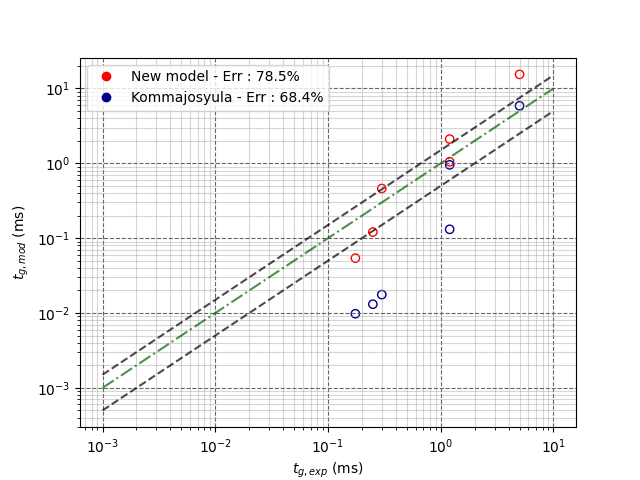
\includegraphics[width=0.6\linewidth]{img/tg/comp_tg_unal.png}
\caption{Comparison of the proposed model and Kommajoyusla model against experimental data from Unal. Black lines represent the $\pm 50\%$ error bars.}
\label{fig:comp_modelKomm}
\end{figure}

As we can see, the average error from our model is greater than Kommajosyula's one. However, this is mainly due to the highest measured growth time (upper right point). Without this measurement, the average error reaches $52.5\%$, indicating that a much greater number of experimental measurements should be needed properly evaluate each model.

\npar
On the other hand, we may consider that the proposed approach could be of interest since it is not based on data-fitted parameters while providing reasonable results.



\begin{table}[h!]

%\begin{changemargin}{-1cm}{0cm}

\noindent\makebox[\textwidth]{

\scriptsize
\centering
\begin{tabular}{p{20mm}|c c c c c c c c} 
Author & Fluid & $D_{h}$ [mm] & $P$ [bar] & $G_{L}$ [$\debm$] & $\Delta T_{L}$ [K] & $\phi_{w}$ [kW/m\up{2}] & $\Delta T_{w}$ [K] & $D_{d}$ [mm] ($N_{mes}$)\\
\hline
\\

Maity \cite{maity_effect_2000} \newline (2000) & Water & 20 & 1.01 & 0 - 239.6 & 0.3 - 0.7 & N.A. & 5 - 5.9 & 0.788 - 1.71 (9) \\

Kossolapov \cite{kossolapov_experimental_2021} \newline (2021) & Water & 20 & 20 - 40 & 500 - 1500 & 0.3 - 0.7 & N.A. & 5 - 5.9 & 0.788 - 1.71 (9) \\

\hline
\end{tabular}
}


\caption{Bubble growth time data in vertical flow boiling}
\label{tab:tg_exp_data}

%\end{changemargin}

\end{table}

\subsection{Bubble Wait Time}

The wait time between two nucleation events on an active site corresponds to the time needed for the thermal boundary layer to reconstruct after its disruption due do bubble departure from the nucleation site.  
\begin{table}[h!]

%\begin{changemargin}{-1cm}{0cm}

\noindent\makebox[\textwidth]{

\scriptsize
\centering
\begin{tabular}{p{20mm}|c c c c c c c c} 
Author & Fluid & $D_{h}$ [mm] & $P$ [bar] & $G_{L}$ [$\debm$] & $\Delta T_{L}$ [K] & $\phi_{w}$ [kW/m\up{2}] & $\Delta T_{w}$ [K] & $D_{d}$ [mm] ($N_{mes}$)\\
\hline
\\

Basu \etal \cite{maity_effect_2000} \newline (2000) & Water & 20 & 1.01 & 0 - 239.6 & 0.3 - 0.7 & N.A. & 5 - 5.9 & 0.788 - 1.71 (9) \\
\\
\hline
\end{tabular}
}

\caption{Bubble wait time data in vertical flow boiling}
\label{tab:tw_exp_data}


%\end{changemargin}

\end{table}



\subsection{Nucleation Site Density}

The Nucleation Site Density is among the most influencing parameters over the HFP models predictions, particularly regarding wall temperature. Indeed, its value directly controls the density of bubbles generated at the heater and therefore impacts both the boiling ($\phi_{e}$) and quenching ($\phi_{q}$) heat fluxes to the first order. Being able to come up with correct predictions of the NSD is thus critical if one wishes to properly capture the thermal behavior of the boiling surface.

However, the value of $N_{sit}$ is actually influenced by many parameters being either linked to thermal-hydraulics (wall temperature, pressure, operating fluid) or the heater material (roughness, wettability). That is why its value is often estimated through empirical correlations, for which many different expression have been proposed over the years since the end of the XX\textsuperscript{th} century.

\npar

One of the firstly identified behavior of the NSD was its power dependency with the wall superheat ($N_{sit} \propto {\Delta T_{w}}^{m}$), which is form adopted in the correlation of Lemmert \& Chawla \cite{Lemmert} : 

\begin{align}
N_{sit}=\crocht{210\parth{T_{w}-T_{sat}}}^{1.8}
\label{eq:nsit_lemmert}
\end{align}

\begin{remark*}{}
This law is used in the HFP model of Kurul \& Podowski and NEPTUNE\_CFD to compute $N_{sit}$.
\end{remark*}

However, such an expression misses the influence of other parameters such as pressure, which has been proven to be strongly impacting the range of active cavities that can generate bubbles as shown on Figure \ref{fig:nsd_P_koss} and induces a larger bubble density over the heater. 

\begin{figure}[h!]
\centering
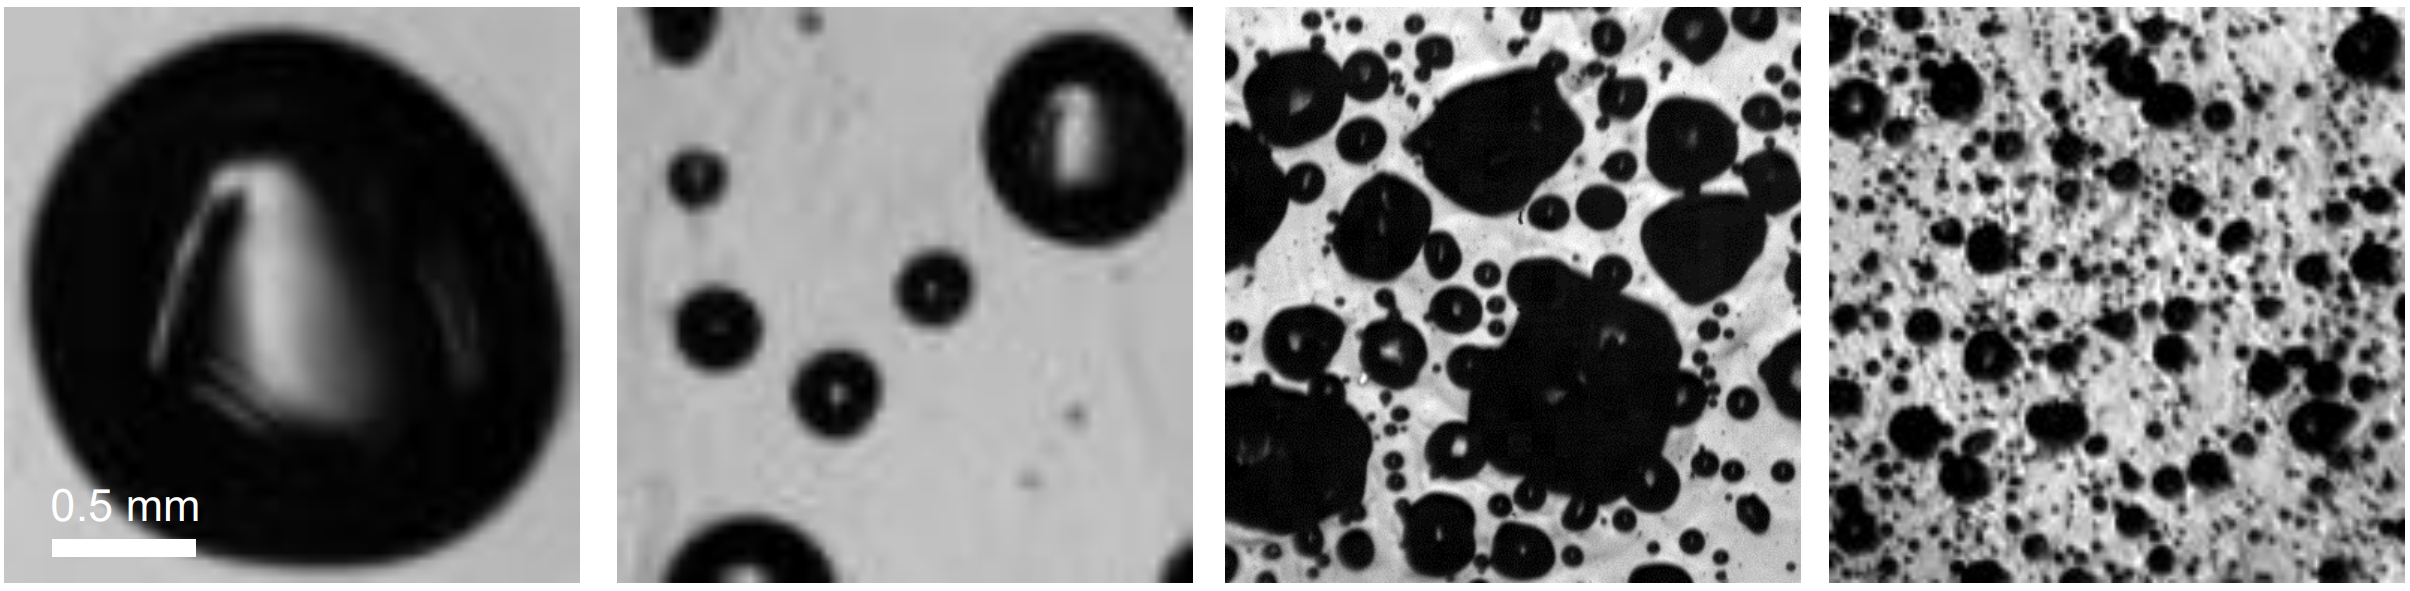
\includegraphics[width=0.7\linewidth]{img/NSD/nsd_press_koss.png}
\caption{HSV Visualization of bubble density at various pressures adapted from Kossolapov \cite{kossolapov_experimental_2021} (left to right: 1.01 bar, 3 bar, 19.8 bar, 75.8 bar). }
\label{fig:nsd_P_koss}
\end{figure}

\npar

Moreover, experimental measurements such as in Borishanskii \cite{borishanskii} showed that the power dependency on the wall superheat changes by increasing both with pressure and the superheat value itself. This was accounted for by Hibiki \& Ishii in 2003 \cite{hibiki_ishii} who came up with a new correlation that requires an estimation of the minimum activated cavity radius $R_{c}$ : 


\begin{align}
N_{sit} =& N_{0}\parth{1-\exp{-\dfrac{\theta^{2}}{8\mu^{2}} } }\crocht{\exp{ \mathrm{f}\parth{\rho^{+}}\dfrac{\lambda '}{R_{c}} } -1}
\label{eq:nsit_hibiki} \\
%
R_{c} =& \dfrac{2\sigma\parth{1+\dfrac{\rho_{V}}{\rho_{L}}} / P }{\exp{\dfrac{h_{LV} \Delta T_{w}}{R_{g}T_{w}T_{sat}} } -1}\\
%
\mathrm{f}\parth{\rho^{+}} =& -0.01064 + 0.48246\rho^{+} - 0.22712 \rho^{+^{2}} + 0.05468 \rho^{+^{3}}
\end{align}
with $R_{g}$ the perfect gas constant times the molar mass of the fluid,  $N_{0}=4.72\times 10^{5}\ \mathrm{m}^{-2}$, $\mu = 0.722\ \mathrm{rad}$, $\lambda ' = 2.5 \times 10^{-3} \ \mathrm{m}$ and $\rho^{+}=\mathrm{log}_{10}\parth{\dfrac{\rho_{L}-\rho_{V}}{\rho_{V}}}$.


\begin{remark*}{}
This law is used in the HFP model of Gilman \& Baglietto \cite{gilman_baglietto}.
\end{remark*}

We can note that it also includes the value of the static contact angle $\theta$ which can be used as a parameter to accounts for wall properties, since it is dependent on the wall roughness, wettability and the operating fluid. 

Indeed, a high-wetting material (low values of $\theta$) will allow smaller cavities to be flooded by the surrounding liquid, thus hindering non-condensable gases to be captured inside and become a potentially active nucleation site (Figure \ref{fig:nsd_theta_wet}).

\begin{figure}[h!]
\centering
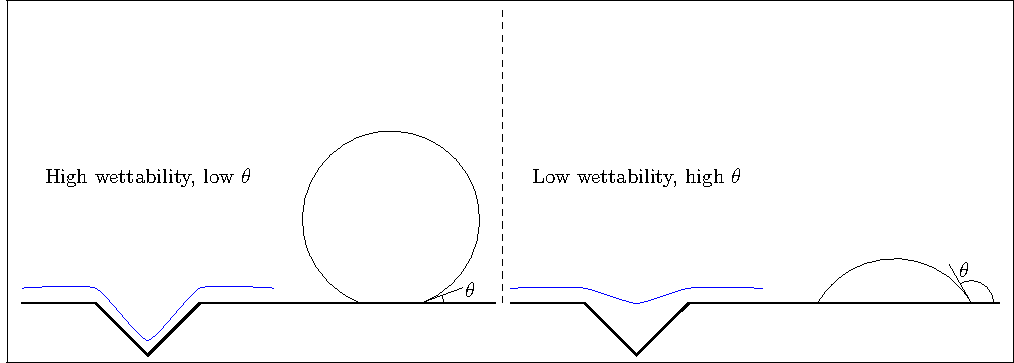
\includegraphics[scale=0.8]{img/NSD/wettability.pdf}
\caption{Sketch of the link between bubble contact angle and wettability / cavity flooding}
\label{fig:nsd_theta_wet}
\end{figure}

This influence of the contact angle on the NSD was confirmed by experimental obervations of Basu \etal \cite{basu_nsit} and was also included in a law correlated on their own measurements :

\begin{align}
N_{sit}=&
\begin{dcases}
0.34\crocht{1-\cos{\theta}} {\Delta T_{w}}^{2} & \text{if } \Delta T_{w,ONB}<\Delta T_{w} < 15\ K\\
3.4\times 10^{-5}\crocht{1-\cos{\theta}} {\Delta T_{w}}^{5.3} & \text{if } \Delta T_{w} > 15\ K
\end{dcases}
\label{eq:nsit_basu}
\end{align}

\npar

Similarly, Zhou \etal \cite{zhou_nsd} correlated their measurements, including an influence of the pressure:

\begin{align}
N_{sit} =& N_{0}\parth{1-\cos{\theta}}\crocht{\exp{\mathrm{f}\parth{P} \Delta T_{w} } -1 }
\label{eq:nsit_zhou}\\
&\mathrm{f}\parth{P} = 0.218~\ln{\dfrac{P}{P_{0}}}+0.1907
\end{align}
with $N_{0}=55~395.26\ \mathrm{m}^{-2}$ and $P_{0}=1.01\ \mathrm{bar}$.

\npar

Finally, one of the most recent NSD correlation has been proposed by Li \etal in 2018 \cite{li_new_2018} and validated over a large range of measurements by including a more realistic power law for $\Delta T_{w}$. It avoids the divergence of $N_{sit}$ observed in Hibiki \& Ishii law (Eq. \ref{eq:nsit_hibiki}) when reaching high pressure and superheats. It also includes the impact of pressure and contact angle and its evolution with temperature \eg its decrease close to 0 $\degree$ when approaching the critical temperature \cite{song_fan_contact_angle}:


\begin{align}
N_{sit} &= N_{0}e^{\mathrm{f}\parth{P}} {\Delta T_{w}}^{A\Delta T_{w} + B} \parth{1- \cos{\theta}}
\label{eq:nsit_li}\\
%
\mathrm{f}\parth{P} &= 26.006 - 3.678 e^{-2P} - 21.907e^{-P / 24.0.65}\\
%
A &= -2\times 10^{-4} P^{2} + 0.0108P + 0.0119\\
%
B &= 0.122P +1.988\\
%
1-\cos{\theta} &= \parth{1-\cos{\theta_{0}}}\parth{\frac{T_{c}-T_{sat}}{T_{c}-T_{0}}}^{\gamma}
\end{align}
with $P$ in MPa, $\theta_{0}$ the contact angle at room temperature $T_{0}$, and default value being for water $\theta_{0}=41.37 \degree$, $T_{c}=374 \degree$C $T_{0}=25\degree$C, $\gamma = 0.719$.

\npar

In order to assess existing NSD correlations and choose the most pertinent to include in a HFP model, we gather NSD measurements from 4 different authors. The different operating conditions of the chosen data sets are gathered on Table \ref{tab:nsit_exp_data}.


\begin{table}[h!]

%\begin{changemargin}{-1cm}{0cm}

\noindent\makebox[\textwidth]{

\scriptsize
\centering
\begin{tabular}{p{20mm}|c c c c c c c c} 
Author & Fluid &  $P$ [bar] & $G_{L}$ [$\debm$] & $\Delta T_{L}$ [K]  & $\Delta T_{w}$ [K] & $\theta_{0}$ &  $N_{mes}$ [-]\\
\hline
\\

Zhou \cite{zhou_nsit} \newline (2020) & Water & 1.21 - 3.12 & 482.7 - 1930.6 & 8 - 15  & 6.7 - 20.2 & $51\degree$ & 60 \\
\\

Richenderfer \cite{richenderfer} \newline (2018) & Water & 1.01 & 500 - 1000 & 10 & 21.7 - 42.8 & $80\degree$ & 49 \\
\\

Kossolapov \cite{kossolapov_experimental_2021} \newline (2021) & Water & 1.01 - 75.8 & 500 - 2000 & $80\degree$ &10 & 0.13 - 30.1 & 63 & \\
\\

Borishanskii \cite{borishanskii} \newline (1966) & Water & 1.01 - 198 & N.A. & N.A. & 1.75 - 17.3 & $45\degree$ & 132 \\
\\

\hline
\end{tabular}
}

\caption{Nucleation Site Density data in flow boiling}
\label{tab:nsit_exp_data}


\end{table}



We then compare the predictions achieved by the model of Lemmert \& Chawla (Eq. \ref{eq:nsit_lemmert}), Hibiki \& Ishii (Eq. \ref{eq:nsit_hibiki}), Zhou \etal (Eq. \ref{eq:nsit_zhou}) and Li \etal (Eq. \ref{eq:nsit_li}).  The comparison with measurements are presented on Figure \ref{fig:pred_nsit_models}.




\begin{figure}[!h]
\centering
\subfloat[Lemmert \& Chawla model]{
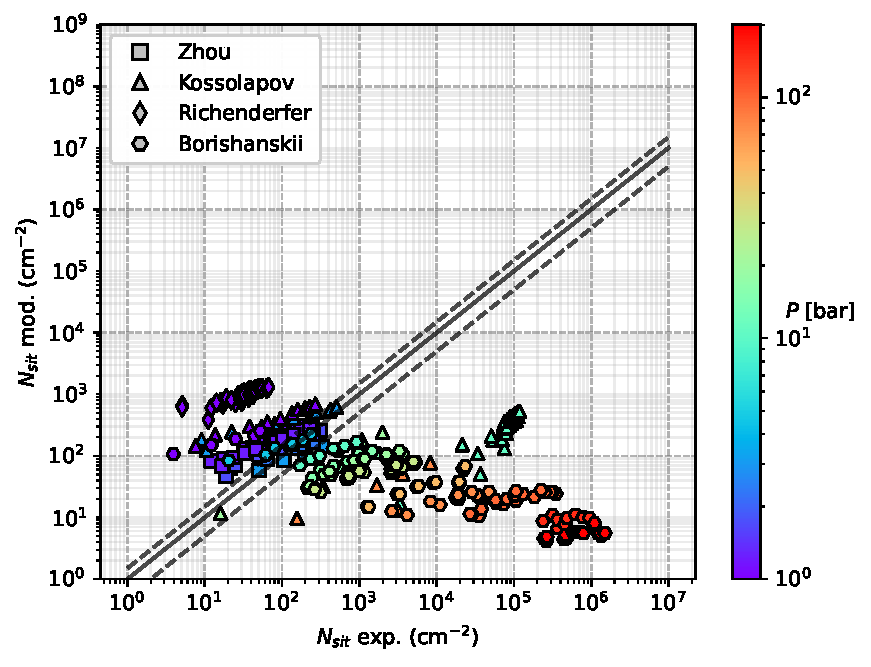
\includegraphics[width=0.45\linewidth]{img/NSD/nsit_LC.pdf}
\label{fig:pred_nsit_lemmert}
} 
\subfloat[Hibiki \& Ishii model]{
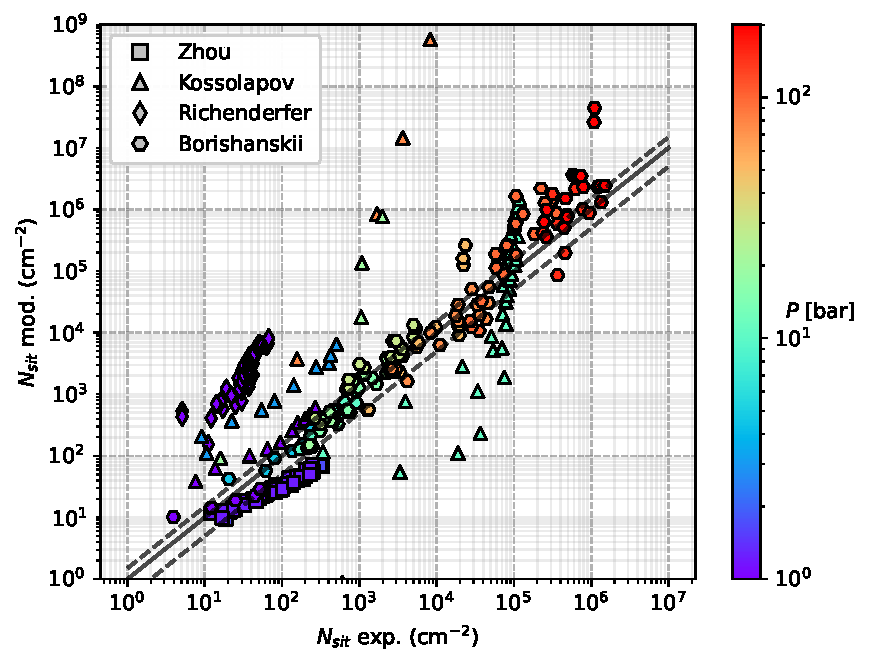
\includegraphics[width=0.45\linewidth]{img/NSD/nsit_HI.pdf}
\label{fig:pred_nsit_hibiki}
}
\\
\subfloat[Zhou \etal model]{
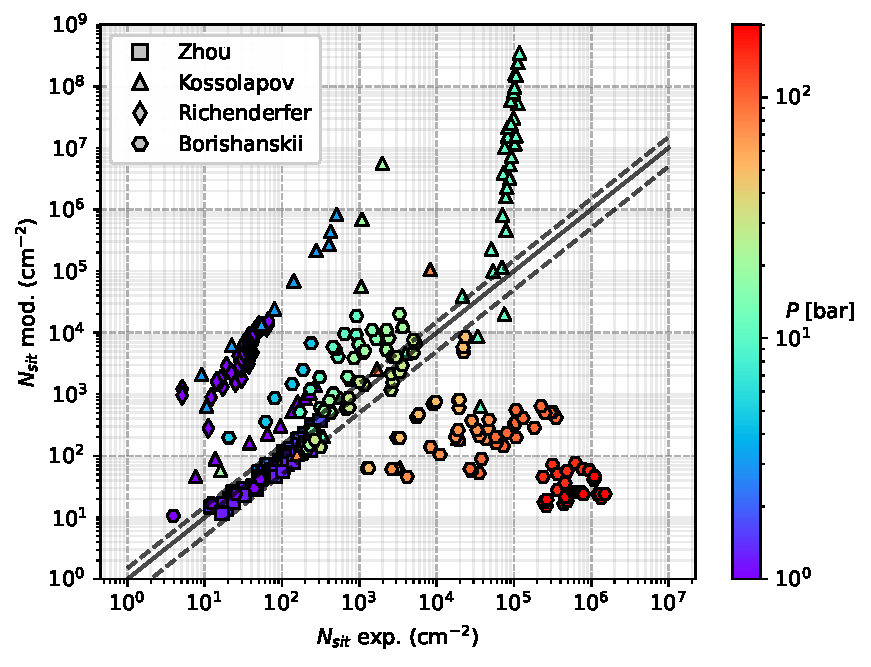
\includegraphics[width=0.45\linewidth]{img/NSD/nsit_Zhou.pdf}
\label{fig:pred_nsit_zhou}
} 
\subfloat[Li \etal model]{
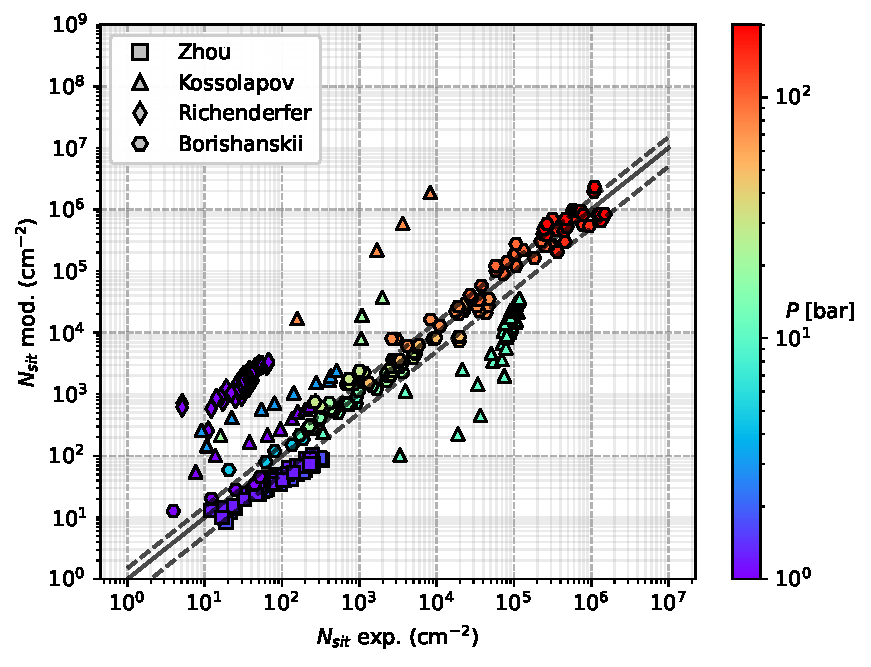
\includegraphics[width=0.45\linewidth]{img/NSD/nsit_Li.pdf}
\label{fig:pred_nsit_li}
}

\caption{Predictions of the chosen models against the experimental data of Table \ref{tab:nsit_exp_data} with $\pm 50\%$ error bars. The contact angles}
\label{fig:pred_nsit_models}
\end{figure}

The Lemmert \& Chawla model appears to fail in predicting the NSD at high pressures. This is a logical drawback of its sole dependence on the wall superheat. More importantly it increasingly underestimates the NSD as pressure increases, which makes it a clearly unsuitable correlation to compute $N_{sit}$ particularly for pressurized flows such as in PWR.

Altough the model of Zhou \etal includes a pressure term, its partial calibration on data covering a low range of pressure may explain the large error observed when compared to higher pressure measurements.

On the contrary, models from Hibiki \& Ishii and Li \etal seem to better reproduce the different trends with flow conditions, especially with pressure. The model from Li \etal achieves better predictions by avoiding to reach unphysically high values of $N_{sit}$ at higher wall superheat compared to Hibiki \& Ishii. This behavior is clear over Kossolapov data at high pressure, where both model lead to overestimations, the strongest discrepancy being associated to Hibiki \& Ishii model.

Overall, the model of Li \etal is the most efficient with an acceptable agreement on most of the data of Borishanskii and Zhou \etal. The measurements of Richenderfer and Kossolapov fail to be precisely reproduced, but it shows a coherent trend and the most limited error when compared to other correlations.

\begin{remark*}{}
The coherency of NSD predictions is hard to ensure since we do not know the exact contact angle and boiling surface morphology in the experiments. In particular, the overpredictions on Richenderfer and Kossolapov data can be reduced by strongly diminishing the contact angle. On the other hand, the fact that the NSD measured by Kossolapov at $10.5$ bar is higher than any other pressure on his experiment is surprising and thus lead to underpredictions of the model of Li \etal
\end{remark*}


All things considered, those comparisons show that the Nucleation Site Density remains among the most difficult quantity to evaluate because of its very large variations over experiments, boiling surfaces and flow conditions. Dedicated correlations are hardly precise outside of their establishment databases. However, it remains the best yet only way to compute $N_{sit}$. \textbf{In that regard, the NSD correlation of Li \etal appears to be the most coherent choice.}


\subsection{Considerations on bubble interaction and nucleation sites deactivation}

NSD correlation actually compute the total number of sites where bubbles can nucleate on a surface. However, they do not represent how important a nucleation site will be in term of bubbles generation compared to another. 

\npar
In fact, Kossolapov has observed that each nucleation site has its own bubble nucleation frequency. Thus implying that some sites play a much greater role in wall nucleation compared to others. One can even consider that some nucleation sites can be neglected regarding their small impact on the whole phase change process.

\npar

In order to physically take into account this effect, Gilman considered a statistical approach, by assuming that nucleation site are randomly distributed over the heater surface (Complete Spatial Randomness). Then, considering that a nucleation site located under a bubble will be deactivated, one can express the number of sites actually contributing to bubble nucleation $N_{sit,a}$ as :


\begin{align}
N_{sit,a}=\parth{1-\mathcal{P}}N_{sit},\ \text{with}\ \mathcal{P}=1-e^{-N_{b}\pi \parth{D_{b}/2}^{2}}
\end{align}
where $N_{b}=t_{g}fN_{sit}$ is the actual average density of bubbles on the heater surface.

\npar

The resulting number of sites is a solution of the implicit equation on $N_{sit}$, which can be solved numerically or using the Lambert function (reciprocal of $w\rightarrow we^{-w}$).

\npar

{\color{red} Je vais détailler un peu plus cela avec des schémas clairs, ainsi qu'un exemple de comment cela pondère la densité de site totale, puisque cela permet d'éviter la divergence dans une loi telle que celle de Hibki \& Ishii à haute surchauffe pariétale} 



\subsection{Nucleation Sites and Bubbles Interactions}


\subsubsection{Static suppression}

If we suppose that the nucleation sites follow a homogeneous spatial Poisson process with an event density $\lambda$, we can express the probability of finding $n$ sites within an area A as :

\begin{align}
\mathcal{P}\parth{N\parth{A}=n}=\frac{\parth{\lambda A}^{n}}{n!}e^{-\lambda A}
\end{align}

If we consider the actual number of bubble-generating sites $N_{b}$, those sites are holding a bubble over a fraction $t_{g}f$ of the nucleation cycles in average. Thus, the actual density of bubbles held by the sites is : $t_{g}f N_{b}$. To derive $N_{b}$ from the value $N_{sit}$ provided by NSD correlations, we have to evaluate the probability of nucleation site overlapping, which corresponds to a distance $r$ lower than $R_{d}$ between two bubbles. 

\begin{align}
\mathcal{P}\parth{r\leq R_{d}} &=1-\mathcal{P}\parth{N\parth{\pi R_{d}^{2}}=0}\\
&=1-e^{-N_{b}t_{g}f\pi R_{d}^{2}} = \mathcal{P}
\end{align}

This probability thus represents the proportion of bubble that can't be geometrically accomodated on the surface. We can then evaluate $N_{b}$ from $N_ {sit}$ as :

\begin{align}
&N_{b}=\parth{1-\mathcal{P}}N_{sit} \\
%
\Leftrightarrow\  &N_{b}t_{g}f\pi R_{d}^{2}e^{N_{b}t_{g}f \pi R_{d}^{2}}= N_{sit}t_{g}f \pi R_{d}^{2} \\
%
\Leftrightarrow\   &N_{b} = \frac{\mathcal{W}\parth{N_{sit}\mathsf{A}}}{\mathsf{A}}\ \ \ \text{where}\ \ \ \mathsf{A}=t_{g}f\pi R_{d}^{2}
\end{align}



\subsubsection{Static coalescence}

Now that the actual number of bubble-generating sites have been identified, we can consider other interaction phenomena that can occur on the boiling surface. For instance, if two sites are simultaneously generating a bubble at a distance $d$ between $R_{d}$ and $2R_{d}$, the bubbles will coalesce while growing up to the detachment diameter. To estimate the probability of having a bubble on a site in this distance range, we consider the probability density function of the nearest-neighbour in the case of a homogeneous spatial Poisson process $f$ with an event density $\lambda$. 

\begin{align}
f\parth{r}=2\lambda \pi r e^{-\lambda \pi r^{2}}
\end{align} 

The considered probability of interaction is then :

\begin{align}
\mathcal{P}\parth{R_{d}\leq r \leq 2R_{d}} &=\int_{R_{d}}^{2R_{d}}f\parth{r} \mathrm{d}r \\
%
&= e^{-\lambda \pi R_{d}^{2}} - e^{-4\lambda \pi R_{d}^{2}}\\
%
&= e^{-\lambda \pi R_{d}^{2}}\crocht{1-\parth{e^{-\lambda \pi R_{d}^{2}}}^{3}} \\
&= \mathcal{P}_{coal,st} \ \ \ \text{with}\ \ \ \lambda=t_{g} f N_{b}
\end{align}

The density of bubble-generating sites that will lead to a static coalescence can then be estimated as :

\begin{align}
N_{coal,st}=\mathcal{P}_{coal,st}N_{b}
\end{align}

If we suppose that coalescing bubbles will instantly lift-off due to the perturbation associated with the coalescence process, this yields an associated boiling flux :

\begin{align}
\phi_{e,coal,st}=N_{coal,st} f \rho_{V}h_{LV} \frac{4}{3}\pi R_{coal,st}^{3} \ \ \ \text{where}\ \ \ R_{coal,st}=\sqrt[3]{2}R_{d} 
\end{align}

considering that the bubbles will merge approximately at $R=R_{d}$.

\subsubsection{Sliding coalescence}

Now that suppressed sites and sites that will lead to static coalescence have been identified, the remaining sites $N_{sl}=\parth{1-\mathcal{P}_{coal,st}}N_{b}$ will generate sliding bubbles. While sliding, a single bubble swipes an area :

\begin{align}
A_{sl, 1b} \approx l_{sl,1b}\frac{D_{d}+D_{lo}}{2}
\end{align}

In this area, there are an average number of bubble-generating sites $N_{b}A_{sl,1b}$ and an average number of growing bubbles on their sites $t_{g}f N_{b}A_{sl,1b}$

\npar
Two situations can happen from the sliding process :

\begin{itemize}
\item The bubble slides without coalescing
\item The bubble coalesces while sliding with a bubble growing on its site and lifts-off
\end{itemize}


Following the same approach from the static suppression, we can estimate the probability of finding no growing bubble over the sliding surface : 

\begin{align}
\mathcal{P}\parth{N\parth{A_{sl,1b}}=0 }=e^{-N_{b}t_{g}fA_{sl,1b}}
\end{align}

Thus, if a sliding bubble among the $N_{sl}$ does not encounter any growing bubble, the sites on its sliding area will be wiped and thus be quenched by cold liquid. This means that those sites will be suppressed due to the sliding of other bubbles over them.

Among the $N_{b}$ bubble generating sites we can identify 4 categories of sites :

\begin{itemize}
\item Sites generating bubbles which will slide without encountering any growing bubble on their path : $$N_{sl, NC}=N_{sl}e^{-ft_{g}N_{b}A_{sl,1b}}$$

\item Sites generating bubbles that will coalesce with a growing bubble during sliding : 
$$N_{sl, C}=  N_{sl}\parth{1-e^{-ft_{g}N_{b}A_{sl,1b}}}$$

\item Sites which will be suppressed by bubbles sliding without coalescing : $$N_{sup, sl}=N_{sl,NC}\ N_{b}A_{sl,1b}$$

\item Sites generating bubbles that will coalesce with a sliding bubble coming from upstream. Those bubbles are still in the growing phase up to detachment when they are coalescing with sliding bubbles. Therefore, there are equal to the number of sliding bubbles that will coalesce : $$N_{g,C}=N_{sl,C}$$

\end{itemize}

This allows to finally write :

\begin{align}
N_{b}&=N_{sl,NC}+N_{sl,C}+N_{sup,sl} + N_{g,C}\\
%
&=N_{sl}\crocht{2-e^{-ft_{g}N_{b}A_{sl,1b}}\parth{A_{sl,1b}N_{b}-1}}
\end{align}

Which finally yields the total number of sliding bubbles : 

\begin{align}
N_{sl}=\frac{N_{b}}{2-e^{-ft_{g}N_{b}A_{sl,1b}}\parth{A_{sl,1b}N_{b}-1}}
\end{align}